\chapter{开放式陆地生态系统碳循环模型对比框架设计}
\label{chap:arch}

陆地生态系统碳循环模型具有种类多样、参数复杂、难以应用的特点,模拟过程参与的要素众多(如GPP、NPP、NEP、Biomass、LAI等),模拟站点丰富,数据需求量大、难以搜集。这些因素都共同阻碍了碳循环模型的应用和发展,开展模型对比工作往往十分艰巨,像CMIP项目那样,各个模式开发组共同参与进来才能更顺利地完成。但是传统的对比框架也面临着一些问题,它将模型计算和对比过程都放在本地计算机运行,模型难以共享和重用,对比过程不够公开,换一套数据或研究区域就难以重现和重复,这些都是由于基于本地计算的对比框架所导致的。针对这一问题,本章旨在设计一个开放式的对比框架,支持将各种对比资源以微服务的形式开放地接入进来,实现可共享、可重用、公开化、易操作的陆地生态系统碳循环模型的对比。

本章首先通过基于微服务的网络架构设计将复杂的系统功能拆分为模型计算层、数据管理层和结果对比层,确保了功能的解耦和系统的稳定;其次为实现三种微服务的管理设计了通用微服务容器,并根据每种微服务的特点在其上扩展,保证了模型对比资源能够以组件的形式接入到系统当中;然后通过对比方案描述语言(CSDL)的设计实现了对比过程的可共享和可重用性;最后通过科学工作流引擎支持网络环境下对比流程地自动化执行。
本系统的整体架构如图\ref{fig:CMIP-architecture}所示。

\begin{figure}[!htbp]
    \centering
    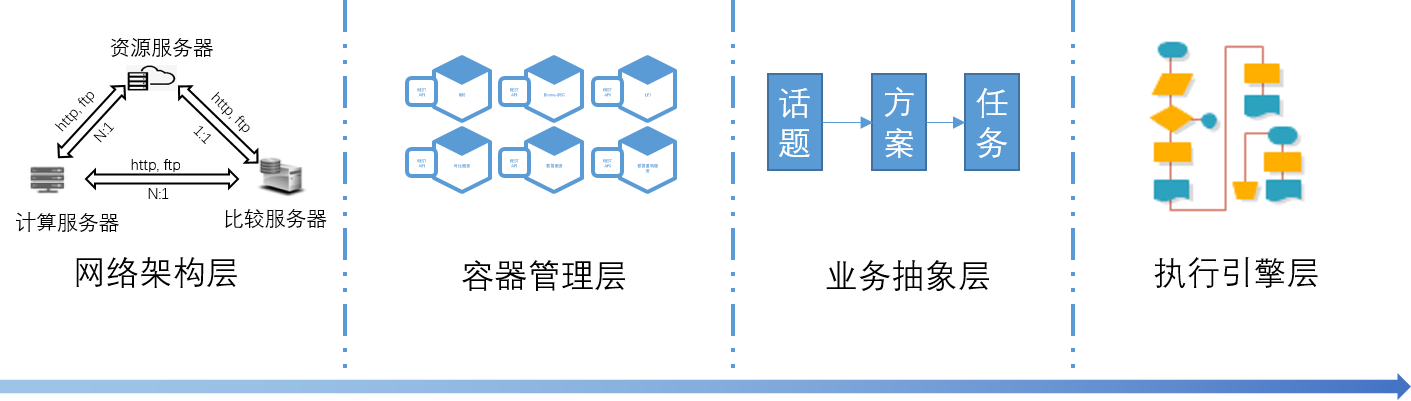
\includegraphics[width=1\textwidth]{CMIP-architecture}
    \caption{陆地生态系统碳循环模型开放式对比框架}
    \label{fig:CMIP-architecture}
\end{figure}

\section{基于微服务的分布式架构设计}
% 开放性应体现在:可共享和重用(业务流程归纳)、计算和对比过程公开化(服务化)、模型和数据资源可扩展(微服务注册和发现)、大规模计算场景下体系稳定可用(微服务LB)、自动化易用(科学工作流)
\subsection{微服务简介与应用}
% 使用原因-引入微服务
% 简介、特点、优点
% 本文应用详细介绍

分布式系统是由一组通过网络进行通信、为了完成共同的任务而协调工作的计算机节点组成的系统。分布式将不同物理区域的计算资源组织整合起来,与传统的集中式相对比,分布式能够有效利用多个分布式节点上的计算能力和数据共享能力,从而提高服务端的性能。
微服务是一种分布式的系统架构风格,由Martin Fowler提出~\cite{fowler2014microservices},微服务是颗粒比较小的服务,服务之间相互独立,具有其独自的数据管理,可以被独立部署,一个大型的复杂软件可以由多个微服务组成。微服务采用UNIX的设计哲学,每种服务只做一件事,是一种松耦合的能够被独立开发和部署的无状态化服务。微服务通过服务来实现应用的组件化,微服务中将组件定义为可被独立替换和升级的软件单元,在应用架构设计中通过将整体应用切分成可独立部署的多个微服务方式进行组件化设计。

\begin{figure}[!htbp]
    \centering
    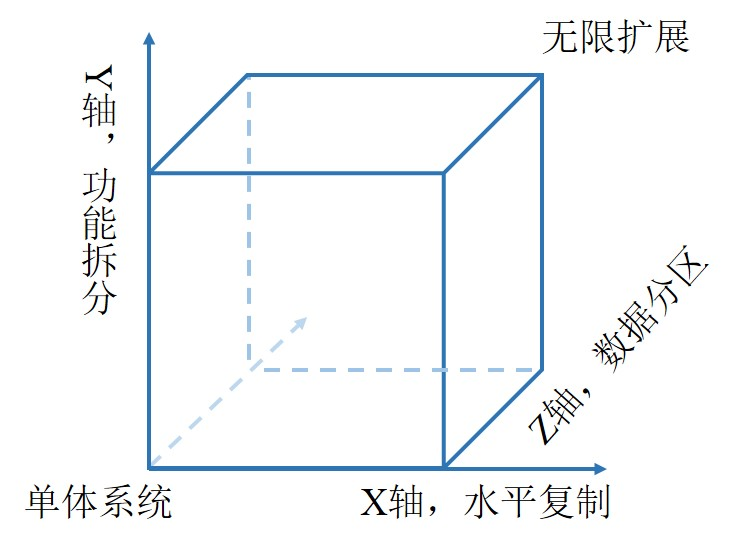
\includegraphics[width=.35\textwidth]{AKF-cube}
    \caption{AKF扩展立方体模型}
    \label{fig:AKF-cube}
\end{figure}

\begin{figure}[!htbp]
    \centering
    \subcaptionbox{微服务应用架构\label{micro-arch}}{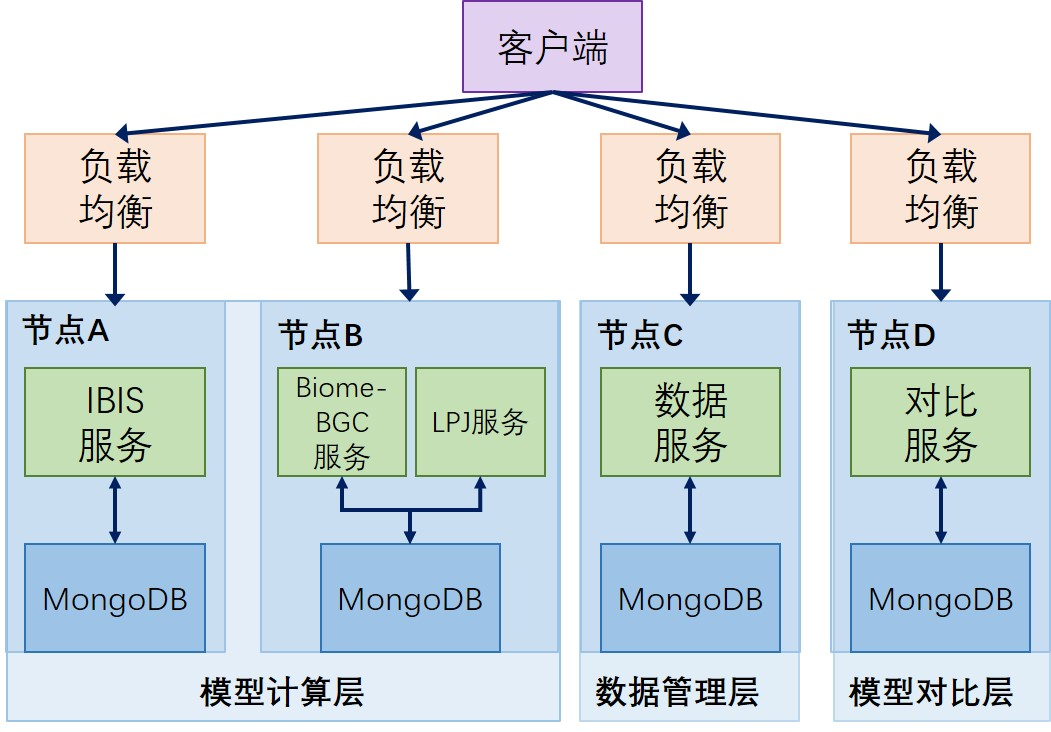
\includegraphics[width=0.6\textwidth]{multi-arch}}
    \hfill
    \subcaptionbox{单体服务应用架构\label{single-arch}}{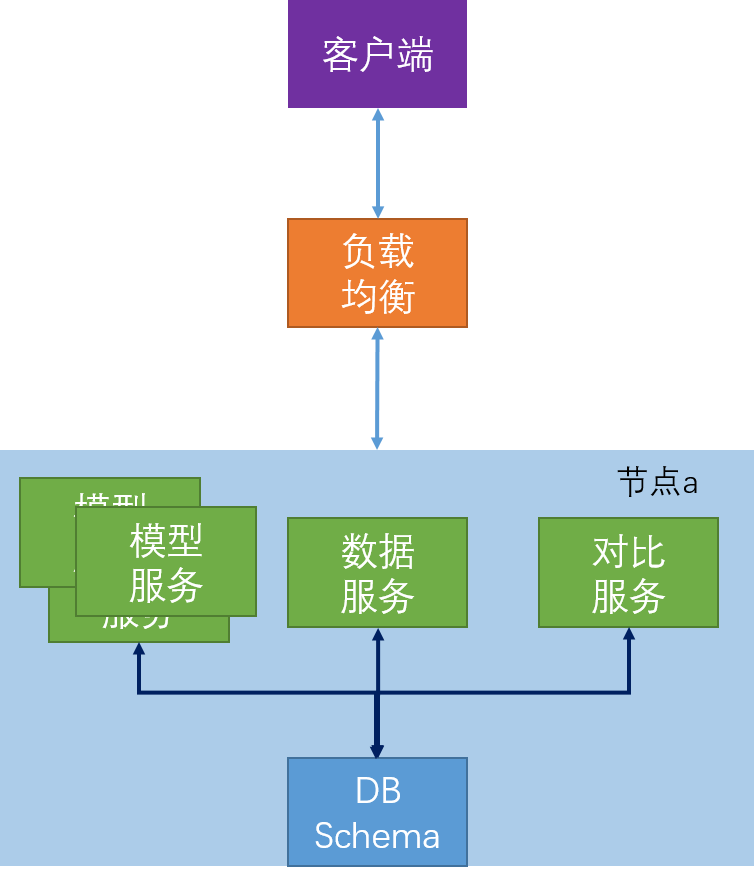
\includegraphics[width=0.35\textwidth]{single-arch}}
    \caption{微服务架构与单体服务架构的对比}
    \label{fig:ms-server-microservice}
\end{figure}

如图~\ref{fig:AKF-cube}所示,微服务的特点可以用AKF立方体~\cite{abbott2009art}表示,应用程序的开发可以抽象为三个维度:

\begin{enumerate}[(1)]
    \item \textbf{X轴:}水平复制。将单体系统运行多个实例,并在其间做负载均衡;
    \item \textbf{Y轴:}功能拆分。基于不同的业务将功能划分为不同的微服务;
    \item \textbf{Z轴:}数据分区。对应用程序的数据库进行拆分,避免遇到数据库瓶颈。
\end{enumerate}

如图~\ref{micro-arch}所示,从Y轴上来看,本文将对比系统的功能拆分为模型计算层、数据管理层和模型对比层;从X轴上来看,将每个功能模块水平复制部署在多个服务器节点上,使用Nginx进行负载均衡;从Z轴来看,每个功能模块独立管理自己的数据库。理论上按照这三个维度的扩展模式,可以将单体系统进行无限扩展,使对比系统面对众多的陆地生态系统碳循环模型和数据资源具有很强的兼容性。三个功能模块都使用微服务实现,其中模型微服务根据模型的软硬件需求,可以将多个模型部署在同一台服务器节点上,也可以分开单独部署,考虑到IBIS模型计算较慢,对软硬件需求较高,本文把他独立部署在一台节点上,而Biome-BGC和LPJ相对来说计算很快,将他们部署在一起。
图~\ref{single-arch}展示了传统的单体服务架构,它将所有功能需求都放在同一台服务器上实现,使得系统庞大臃肿,任意模块一旦崩溃都会引起整个系统的崩溃,而与之相比微服务效率高、灵活性强、可用性高、可扩展性强。

\subsection{微服务治理}
微服务通过功能分解为系统带来无限扩展的可能,同时在集成时也面临着一系列的问题,比如如何发现服务?如何统一对服务进行认证管理?如何针对对比需求进行服务集成?这些都是需要解决的问题。
\subsubsection{动态服务注册与发现}
对于传统的单体应用来说,彼此之间耦合关系较少,通过手动配置IP地址和端口就能满足需求,但是在微服务架构下,服务提供者会不断扩展而变得越来越多,手动配置的方式并不适用于此,而是通过服务注册来解决。本文设计的注册分两个层级,如图~\ref{fig:service-registe-discover}所示,第一级是在计算节点内部的注册,在本级上的注册和注销是服务器管理员对服务进行的管理操作,由计算节点自己独立管理,比如模型计算节点可以发布一个或多个模型服务,也可以注销某些模型服务;第二级是将计算节点注册到中心服务器的数据库中,是将计算节点共享出来以允许服务集成的管理操作。在计算节点启动时,自动向中心服务节点发送注册消息,并持续发送心跳请求,当计算节点宕机或手动注销时,心跳请求停止,中心服务器就能够实时更新出注册的节点列表以及其承载的计算服务。对于处于客户端的用户来说,中心服务器上的服务资源总是最新的和可用的。

\begin{figure}[!htbp]
    \centering
    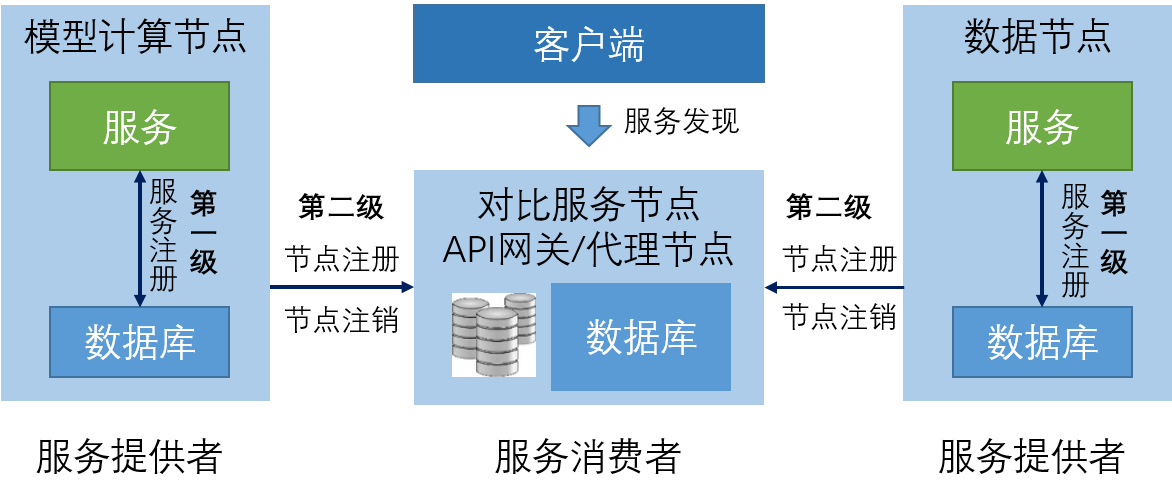
\includegraphics[width=.9\textwidth]{service-registe-discover}
    \caption{动态服务注册与发现}
    \label{fig:service-registe-discover}
\end{figure}

\subsubsection{API网关}
API网关也是针对微服务而出现的技术手段,在单体应用中,客户端需要请求的后台服务器只有一台,而微服务架构下,需要连接的后台节点就多种多样了,他们往往具有异构的接口、协议,以及许多重复化的功能单元,这大大增加了客户端处理逻辑的复杂度。如图~\ref{fig:API-gateway},API网关的设计则是在这些服务节点之上做出一次代理或简单处理,从而屏蔽微服务之间的异构性,使客户端感觉不到微服务的存在。
% TODO 详细说明
在本系统中,API网关的作用主要体现在三点:微服务负载均衡、微服务权限认证和微服务集成。在模型微服务上通过Nginx进行负载均衡管理,使模型微服务在全球共40595个网格点的计算量下保持稳定性和可用性。通过对服务的访问权限控制避免服务受到恶意攻击。API网关上还对服务进行集成整合,满足模型集成对比的需求。

\begin{figure}[!htbp]
    \centering
    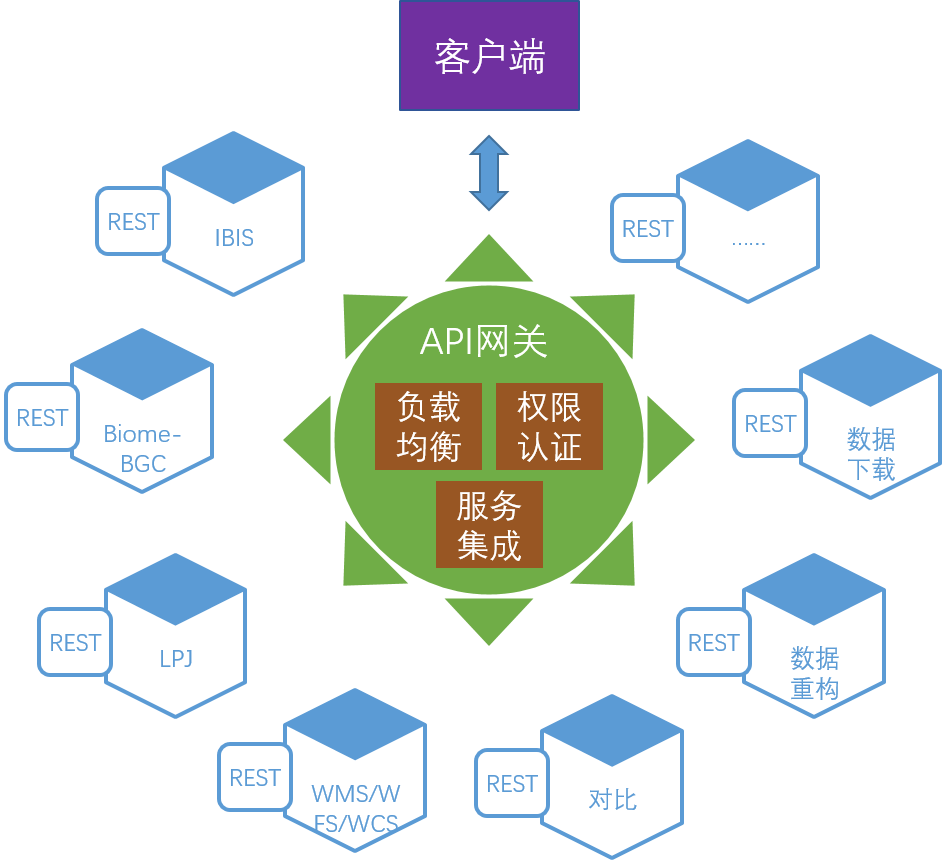
\includegraphics[width=.6\textwidth]{API-gateway}
    \caption{API网关}
    \label{fig:API-gateway}
\end{figure}

% \begin{figure}[!htbp]
%     \centering
%     \subcaptionbox{API网关\label{fig:API-gateway}}{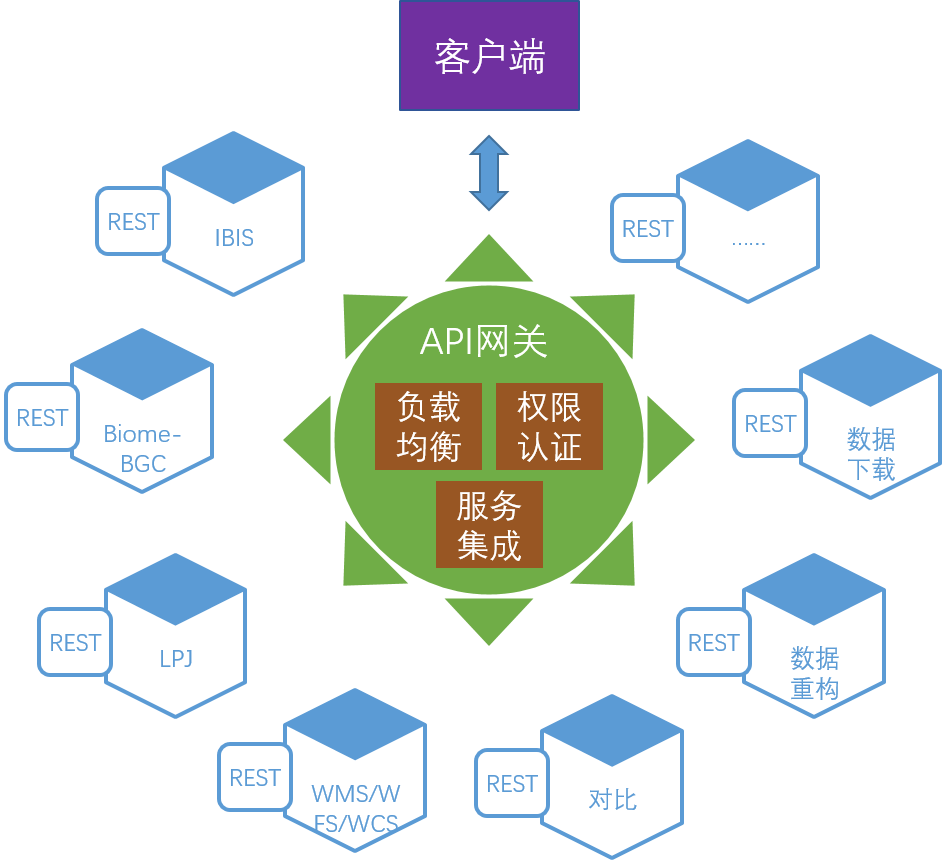
\includegraphics[width=0.6\textwidth]{API-gateway}}
%     \hfill
%     \subcaptionbox{单体服务应用架构\label{fig:no-API-gateway}}{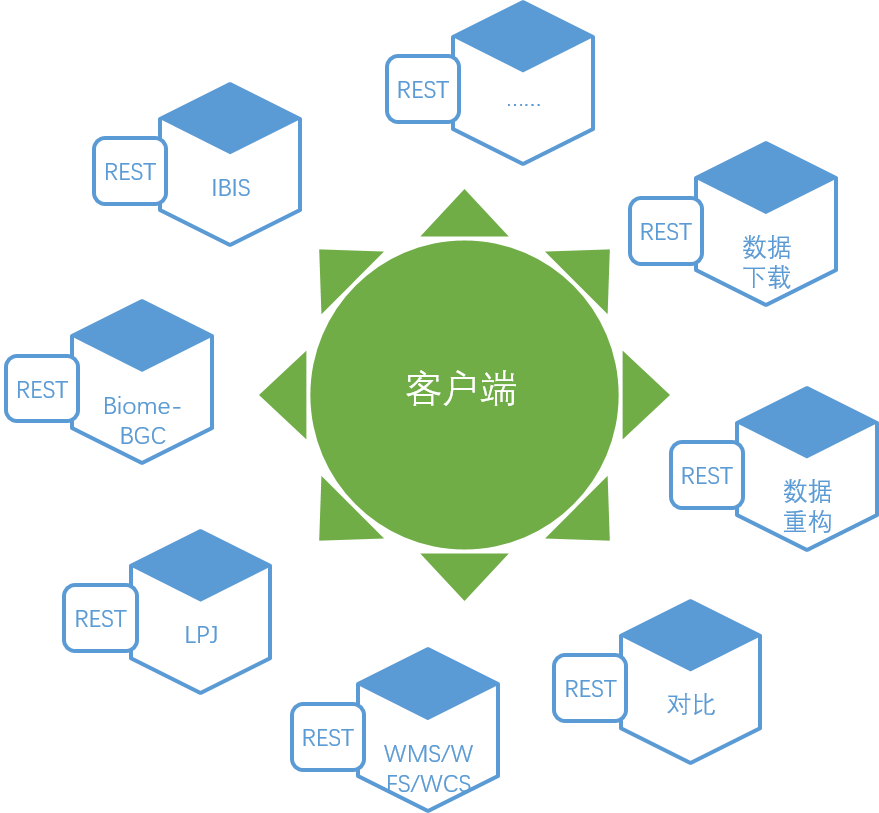
\includegraphics[width=0.35\textwidth]{no-API-gateway}}
%     \caption{}
%     \label{fig:ms-server-microservice}
% \end{figure}

\section{微服务容器和地理资源组件库}
本文将微服务容器定义为微服务的承载工具,微服务容器将经过标准化封装的地理资源组件通过REST API暴露出来,提供了从客户端访问这些组件的能力。根据本文对系统功能的划分,将微服务容器划分为三种:数据管理容器、模型计算容器和模型对比容器,如图~\ref{fig:universe-micro-service-container}所示,三种容器有部分通用的功能,包括微服务发布和注销、微服务运行实例管理、消息通知和日志记录、服务器性能监控等,如果没有统一的微服务管理容器,则这些功能在每个微服务组件中都需要建设一遍,而且对外接口变得五花八样,对于API网关来说难以集成。因此,本文通过通用的微服务容器对微服务进行管理。并在其基础上,针对三种微服务的特点,构建了三种各具特色的微服务容器,以实现三类地理资源组件的微服务发布。

\begin{figure}[!htbp]
    \centering
    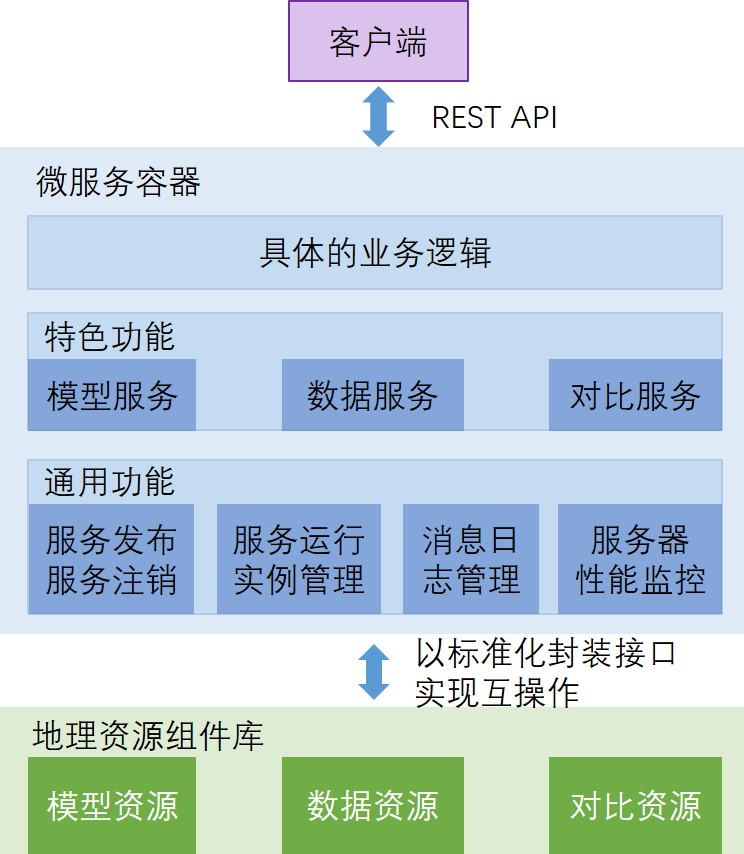
\includegraphics[width=.7\textwidth]{universe-micro-service-container}
    \caption{通用微服务容器设计}
    \label{fig:universe-micro-service-container}
\end{figure}

\subsection{模型计算容器及模型资源组件库}
\subsubsection{模型计算容器}
\begin{figure}[!htbp]
    \centering
    \subcaptionbox{模型微服务的发布和调用}{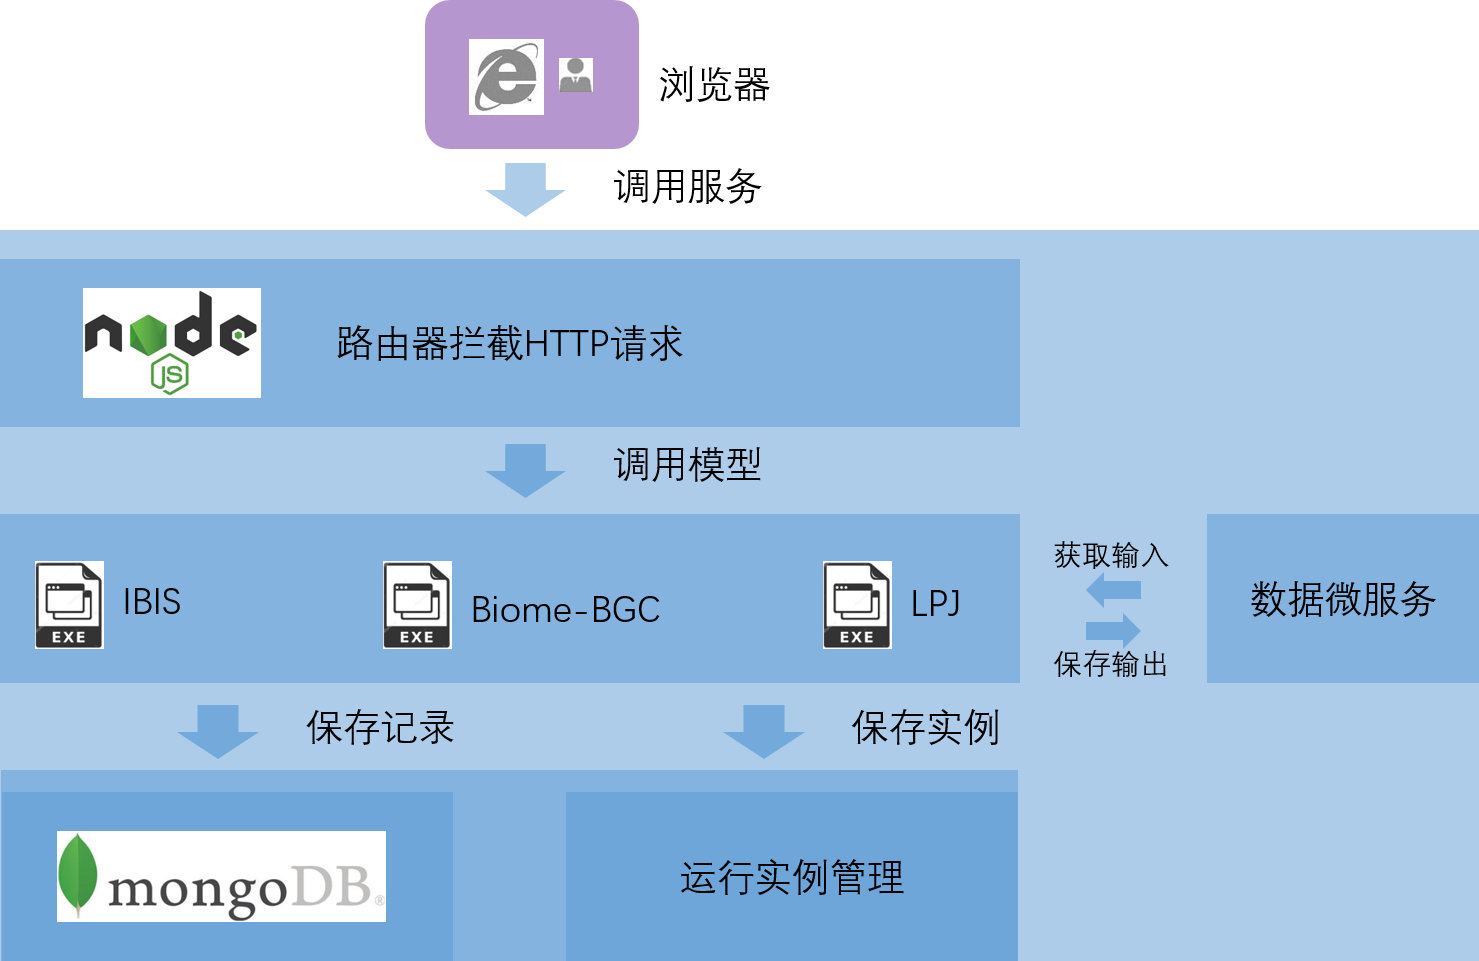
\includegraphics[width=0.7\textwidth]{ms-publish}}
    \hfill
    \subcaptionbox{模型微服务的多节点分布特性}{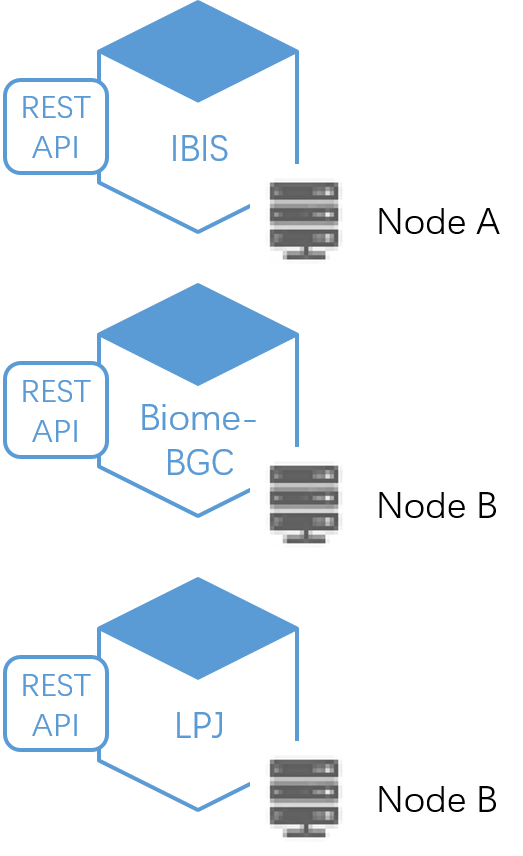
\includegraphics[width=0.25\textwidth]{ms-server-microservice-multi-nodes}}
    \caption{模型计算容器微服务}
    \label{fig:ms-server-microservice}
\end{figure}

模型计算容器对外提供模型计算服务,在传统的本地计算模式下,地理模型操作通常包括运行环境配置、数据准备、启动模型、查看运行进度和输出数据等过程。在网络环境下,模型计算容器通过网络空间向用户提供模型计算功能,其应用模式如图~\ref{fig:model-operation}表示,共包括7步:
\begin{enumerate}[(1)]
    \item 查询所有模型服务列表;
    \item 查看需要运行的模型服务详情,包括模型介绍信息、模型输入数据信息等;
    \item 配置数据,选择服务器上已经存在的数据,或上传用户自己的数据;
    \item 发送异步请求,开始模型运行;
    \item 查看模型调用记录,返回模型的所有运行记录列表;
    \item 查看模型运行状态,返回模型运行的进度以及成功与否;
    \item 下载运行结果。
\end{enumerate}

这个交互模型可以简化为“数据上传——模型计算——结果下载”三部分,其中最核心的功能是第4步,即模型服务的执行,如图~\ref{fig:ms-server-microservice}所示,模型计算容器由Node.js和MongoDB开发。Node.js对外暴露模型调用的接口,当客户端经过HTTP协议发送调用请求时,Node.js拦截到HTTP请求,调用起服务对应的模型可执行程序,模型启动运行前先从数据微服务处获取输入数据,当所有数据准备完成时就开始运行计算。模型计算容器将运行记录和运行实例保存在数据库中,以方便结果查询和实例管理。模型微服务根据软硬件需求可以存放在不同的服务器上,即模型微服务有多个计算节点。

\begin{figure}[!htbp]
    \centering
    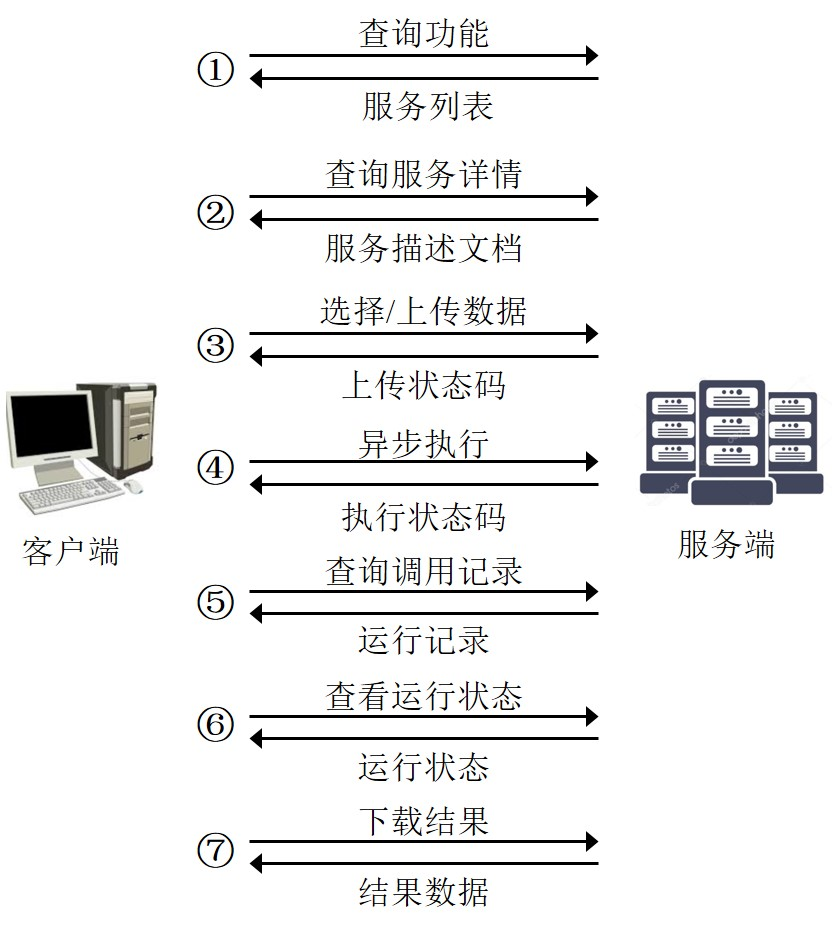
\includegraphics[width=.8\textwidth]{model-operation}
    \caption{模型服务交互模型}
    \label{fig:model-operation}
\end{figure}

\subsubsection{模型资源组件库}

\begin{table}[!htbp]
    \centering
    \caption{模型服务API}
    \label{tab:model-service-API}
    \begin{tabular}{llll}
        \Xhline{1.5pt}
        名称 & 请求方式 & 返回 & 说明 \\
        \Xhline{1.5pt}
        /model-service & GET & 模型服务列表 & 查询模型服务 \\
        /model-service/:msId & GET & 模型描述文档 & 查询模型详情 \\
        /model-service/:msId/invoke & POST & 状态码 & 运行模型 \\ 
        /model-service/records & GET & 运行记录列表 & 查询模型运行记录 \\
        /model-service/records/:recordId & GET & 运行记录 & 查询运行记录 \\
        \Xhline{1.5pt}
    \end{tabular}
\end{table}

\begin{table}[!htbp]
    \centering
    \caption{模型调用接口请求参数}
    \label{tab:model-invoke-API}
    \begin{tabular}{lp{.6\textwidth}l}
        \Xhline{1.5pt}
        参数 & 结构 & 描述 \\
        \Xhline{1.5pt}
        inputs 
        & 
\begin{tabminted}[tabsize=4]{js}
{
  "id": "IO_flag", 
  "value":"uploaded_data_id",
  "description": ""
}[]
\end{tabminted}
        & 输入数据列表 \\
        \hline
        parameters 
        &
\begin{tabminted}[tabsize=4]{js}
{
  "id": "IO_flag", 
  "value": "parameter_value",
  "description": ""
}[]
\end{tabminted}
        & 参数列表 \\
        \hline
        outputs 
        &
\begin{tabminted}[tabsize=4]{js}
{ 
  "id": "IO_flag", 
  "value": null ,
  "description": ""
}[]
\end{tabminted}
        & 输出数据列表 \\
        \Xhline{1.5pt}
    \end{tabular}
\end{table}
模型计算容器所承载的众多模型微服务共同组成模型资源组件库,模型资源组件作为模型对比的参与者,在对比框架下具有形同的角色和地位。与封装之前的模型相比,屏蔽了其在调用接口、实现方法、开发语言等方面的异构性。
模型资源组件库通过表述性状态转移(Representational State Transfer,REST)风格的接口暴露出来,以HTTP请求的POST、DELETE、GET和PUT方法对组件资源进行增删查改操作~\cite{fielding2000architectural}。其详细接口设计如表~\ref{tab:model-service-API}所示,分别对应图~\ref{fig:model-operation}的第1、2、4、5、6步(第3、7步对应数据操作接口)。其中模型调用接口“/model-service/:msId/invoke”是最重要的,其请求参数如表~\ref{tab:model-invoke-API}所示,在调用时,需要在请求体中附加模型的输入项、参数项、输出项,其id表示数据项标识,从“/model-service/:msId”接口返回的描述文档中可以获取,输入项的“value”是上传到服务器的数据id,参数项的“value”是Number或String类型的值,输出项的“value”不用填写。发送请求后,如果调用成功,则返回运行记录的recordId,凭此recordId可以通过“/model-service/records/:recordId”接口请求模型的运行记录,并从中获取运算的结果。

\subsection{数据管理容器及数据资源组件库}
\subsubsection{数据管理容器}
数据管理容器对外提供数据微服务,主要包括以下两点功能:
\begin{enumerate}[(1)]
\item \textbf{数据存储和结果缓存:}数据资源包括各种模型输入数据、对比参照数据和输出数据。模型在运行时从数据管理容器请求输入数据,运行结束后将输出数据存储到数据管理容器。对比任务执行时从数据管理容器请求模型输出数据和对比参考数据,并将对比结果存储到数据服务容器;
\item \textbf{数据服务的发布:}包括WMS、WFS、WCS、数据上传和下载服务、数据重构服务,具体参考第~\ref{sec:data-service}节。
\end{enumerate}

数据管理容器的硬件配置要求是硬盘大,网络带宽高,以方便数据存储和交换。

\subsubsection{数据资源组件库}
\noindent\begin{table}[!htbp]
    \centering
    \caption{数据服务API}
    \label{tab:data-service-API}
    \begin{tabular}{llll}
        \Xhline{1.5pt}
        名称 & 请求方式 & 返回 & 说明 \\
        \Xhline{1.5pt}
        /data & POST & 状态码和数据id & 上传数据 \\
        /data & GET & \multicolumn{1}{m{0.24\columnwidth}}{数据列表,按一定的分类体系组织} & 获取数据列表 \\
        /data/:dataId & GET & 数据文件 & 下载数据 \\
        /data/:dataId/metadata & GET & 元数据文档 & 获取元数据 \\
        /data-refactor & GET & 数据重构服务列表 & \multicolumn{1}{m{0.18\columnwidth}}{查询数据重构服务} \\
        /data-refactor/:id & GET & 重构服务描述 & \multicolumn{1}{m{0.18\columnwidth}}{查询重构服务详情} \\
        /data-refactor/:id/invoke & POST & \multicolumn{1}{m{0.24\columnwidth}}{状态码:200成功,500失败} & 运行重构服务 \\
        /data-refactor/records & GET & 运行记录列表 & \multicolumn{1}{m{0.18\columnwidth}}{查询重构服务运行记录} \\
        /data-refactor/records/:recordId & GET & 运行记录详情 & 查询运行记录 \\
        \Xhline{1.5pt}
    \end{tabular}
\end{table}
数据服务资源库由数据上传下载服务、数据重构服务和OGC WMS、WFS、WCS三类组成。其中数据下载服务将数据按照多种分类体系发布出去,并提供数据的相关元数据描述文档。数据在模型运行和对比时,往往并不能直接驱动程序的运行,数据重构服务对数据做出转换,它的调用交互模式和模型服务的调用类似,表~\ref{tab:data-service-API}列出了数据服务的详细接口,其中“/data-refactor/:id/invoke”的请求体结构和模型服务调用的请求体一致,OGC WMS、WFS、WCS服务的接口和发布在后文第~\ref{subsubsec:OGC}节详细介绍。

\subsection{模型对比容器及对比资源组件库}
\subsubsection{模型对比容器}
对比服务容器的主要功能是将对比任务中包含的计算任务分发给模型计算容器,并把模型计算出来的结果文件和对比参考数据进行对比。对比服务容器在物理实体上也是API网关,他是模型微服务和数据微服务的消费者、对比微服务的生产者。如图~\ref{fig:compare-server-microservice}所示,模型对比的开展主要包括以下几步:

\begin{enumerate}[(1)]
\item 用户在浏览器客户端通过HTTP协议发送对比任务的调用请求;
\item Node.js的路由器收到请求后,将对比任务中包含的计算任务拆分出来,并通过调用模型计算容器上的模型微服务启动计算任务,并不断轮询监控模型的运行进度;
\item 当模型微服务运行成功后,将运行结果提交给数据微服务;
\item 当检测到所有模型都运行成功后,从数据管理容器上获取模型运行结果和对比参考数据,然后启动对比微服务应用程序脚本,这些脚本可由JavaScript、Python或Matlab等编写而成;
\item 最后将对比脚本的结果文件保存到数据库中,并返回给客户端。
\end{enumerate}

另外他作为门户网站的后台服务器,还负责浏览器前台的一系列操作,如资源汇总与展示、对比流程的创建、对比结果的展示等。

\begin{figure}[!htbp]
    \centering
    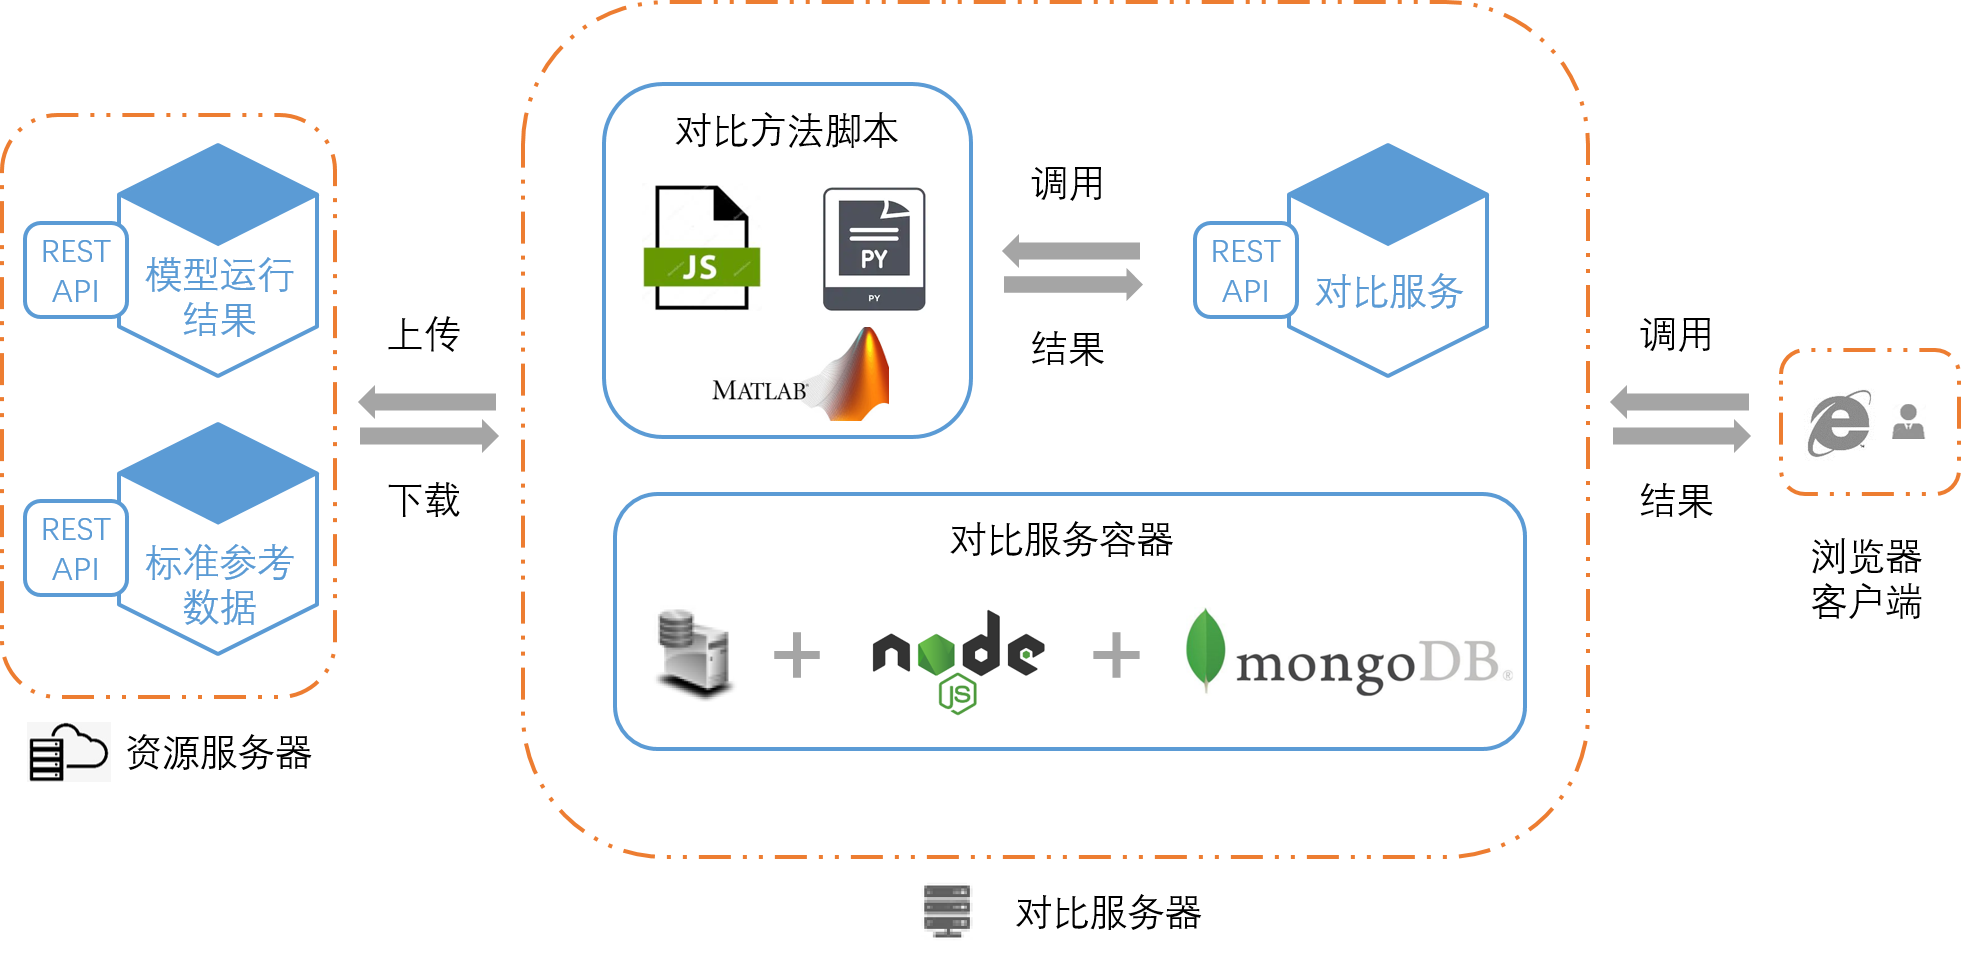
\includegraphics[width=1\textwidth]{compare-server-microservice}
    \caption{对比服务器微服务}
    \label{fig:compare-server-microservice}
\end{figure}

\subsubsection{单位量纲资源库}
在对比服务容器上,设计了单位量纲库对碳循环要素的语义信息进行描述。在多个模型的输出量之间开展对比时,模拟数据和观测数据的单位量纲一般不完全相同,以GPP为例,IBIS的输出单位是$gC m^{-2} d^{-1}$,Biome-BGC的输出单位是$kgC m^2 d^{-1}$,观测数据的单位是$gC m^{-2} d^{-1}$,在对比时,需要将单位一致化,单位量纲资源库为单位转换提供统一参考。
单位量纲资源库由模型运算过程中涉及到的单位和量纲组成,如图~\ref{fig:ModelComparison!3-2-unit-dimension_5}所示,量纲类Dimension由7个基本物理量组成,他们分别是长度($L$)、质量($M$)、时间($T$)、电流($I$)、温度($\Theta$)、物质的量($N$)、发光强度($J$)。而单位类Unit则由这7个基本物理量组合表示(对于无量纲的单位为空),它也可以是自定义的单位。在对比要素类ComparisonFeature中用单位来表达它的具体物理意义,对于不同的单位表示法,可以通过量纲分析进行换算。单位量纲只有一个接口,以GET方式请求“/metrics”可以获取单位量纲列表。表~\ref{tab:std-metrics}列出了本文涉及到的碳循环对比要素及其所使用的单位。

\begin{figure}[!htbp]
    \centering
    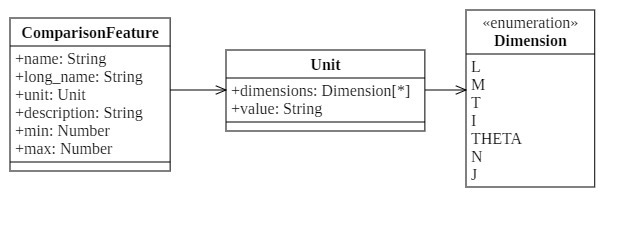
\includegraphics[width=.9\textwidth]{jpg/ModelComparison!3-2-unit-dimension_5}
    \caption{单位量纲UML图}
    \label{fig:ModelComparison!3-2-unit-dimension_5}
\end{figure}

% TODO min and max
\begin{table}[!htbp]
    \caption{对比要素及其单位量纲}
    \label{tab:std-metrics}
    \begin{subtable}[t]{.6\linewidth}
        \centering
        \caption{陆地生态系统碳水循环要素表}
        \label{tab:c-w-feature}
        \begin{tabular}{llrrr}
            \Xhline{1.5pt}
            \textbf{名称} & \textbf{单位} & \textbf{最小值} & \textbf{最大值}  \\
            \Xhline{1.5pt}
            $GPP$ & $gC m^{-2} d^{-1}$ & 0 & 30 \\
            $NPP$ & $gC m^{-2} d^{-1}$ & 0 & 30 \\
            $NEP$ & $gC m^{-2} d^{-1}$ & -30 & 30 \\
            $NEE$ & $gC m^{-2} d^{-1}$ & -30 & 30 \\
            $Biomass$ & $gC m^{-2} d^{-1}$ & 0 & - \\
            $R_A$ & $gC m^{-2} d^{-1}$ & 0 & 30 \\
            $R_H$ & $gC m^{-2} d^{-1}$ & 0 & 30 \\
            $ET$ & $mm d^{-1}$ & 0 & 30\\
            $Runoff$ & $mm d^{-1}$ & - & - \\
            $LAI$ & $m^2/m^2$ & 0 & 1 \\
            \Xhline{1.5pt}
        \end{tabular}
    \end{subtable}%
    \begin{subtable}[t]{.3\linewidth}
        \centering
        \caption{单位量纲表}
        \label{tab:unit-dimension}
        \begin{tabular}{ll}
            \Xhline{1.5pt}
            \textbf{单位} & \textbf{量纲}  \\
            \Xhline{1.5pt}
            \multirow{3}{*}{$gC m^{-2} d^{-1}$} & 质量($M$) \\
            & 长度($L$) \\
            & 时间($T$) \\
            \hline
            \multirow{3}{*}{$kgC m^{-2} y^{-1}$} & 质量($M$) \\
            & 长度($L$) \\
            & 时间($T$) \\
            \hline
            \multirow{2}{*}{$mm d^{-1}$} & 长度($L$) \\
            & 时间($T$) \\
            \Xhline{1.5pt}
        \end{tabular}
    \end{subtable}
\end{table}

\subsubsection{对比服务资源库}
对比服务资源库包括统计学对比方法和可视化对比方法。他们都接受一条或多条数据为输入,统计学对比方法返回的是统计指标,可视化对比方法返回的是图片结果。表~\ref{tab:cmp-service-API}列出了去详细接口,其调用模式与模型微服务一致。

\begin{table}[!htbp]
    \centering
    \caption{对比服务API}
    \label{tab:cmp-service-API}
    \begin{tabular}{llll}
        \Xhline{1.5pt}
        名称 & 请求方式 & 返回 & 说明 \\
        \Xhline{1.5pt}
        /cmp & GET & 对比服务列表 & 查询对比服务 \\
        /cmp/:cmpId & GET & 对比服务描述文档 & 查询对比服务详情 \\
        /cmp/:cmpId/invoke & POST & 状态码 & 运行对比服务 \\ 
        /cmp/records & GET & 对比记录列表 & 查询对比服务运行记录 \\
        /cmp/records/:recordId & GET & 对比结果 & 查询对比结果 \\
        \Xhline{1.5pt}
    \end{tabular}
\end{table}

\section{可共享和重用的对比方案设计}
\label{sec:cmp-CSDL}
针对第\ref{sec:cmp-sln-analysis}节的分析,模型对比通常面临着几个维度上的重用需求:
\begin{enumerate}[(1)]
    \item 在各种研究情景下可重用,包括有历史模拟情景、未来预测情景、敏感性分析情景和参数校准情景等;
    \item 在对比参与者上可扩展,当加入新的模型时可重用;
    \item 在不同的站点和区域上可重现,即在驱动数据配置上可替换。
\end{enumerate}

针对这些重用需求,本文将对比流程设计为三步:“对比话题——对比方案——对比任务”,并设计了对比方案描述语言(Comparison Solution Description Language,CSDL),来描述和表达对比流程,如图~\ref{fig:ModelComparison!3-1-topic-solution-task_3}:

ComparisonTopic表示\textbf{对比话题},它包含了一系列对比要素(ComparisonFeature),并使用desc和wiki字段描述具体的研究问题、对比情景等。

ComparisonSolution表示\textbf{对比方案},它配置了对比参与者(ComparisonService)和使用的对比方法(ComparisonMethod),同样使用desc和wiki字段详细描述方案的配置。对比方案不包括具体的输入数据、观测数据和结果数据,他表示的仅仅是对比的配置项,从而实现对比过程的可共享性、可重用性和可重现性。

ComparisonTask表示\textbf{对比任务},它由一系列模型计算任务(CalculationTask)组成,每个模型计算任务中配置了其所需的输入项和参数项。对比任务是可执行的实体,在启动对比时通过科学工作流执行引擎驱动其运行,并实时更新其运行状态(OGMSState)。对比任务实现了在不同站点和区域上的可重用性。

对比话题、对比方案和对比任务的描述文档都包含了创建者(User)和用户交流记录(Conversition),从而更详细地对对比流程进行解释。

\begin{figure}[!htbp]
    \centering
    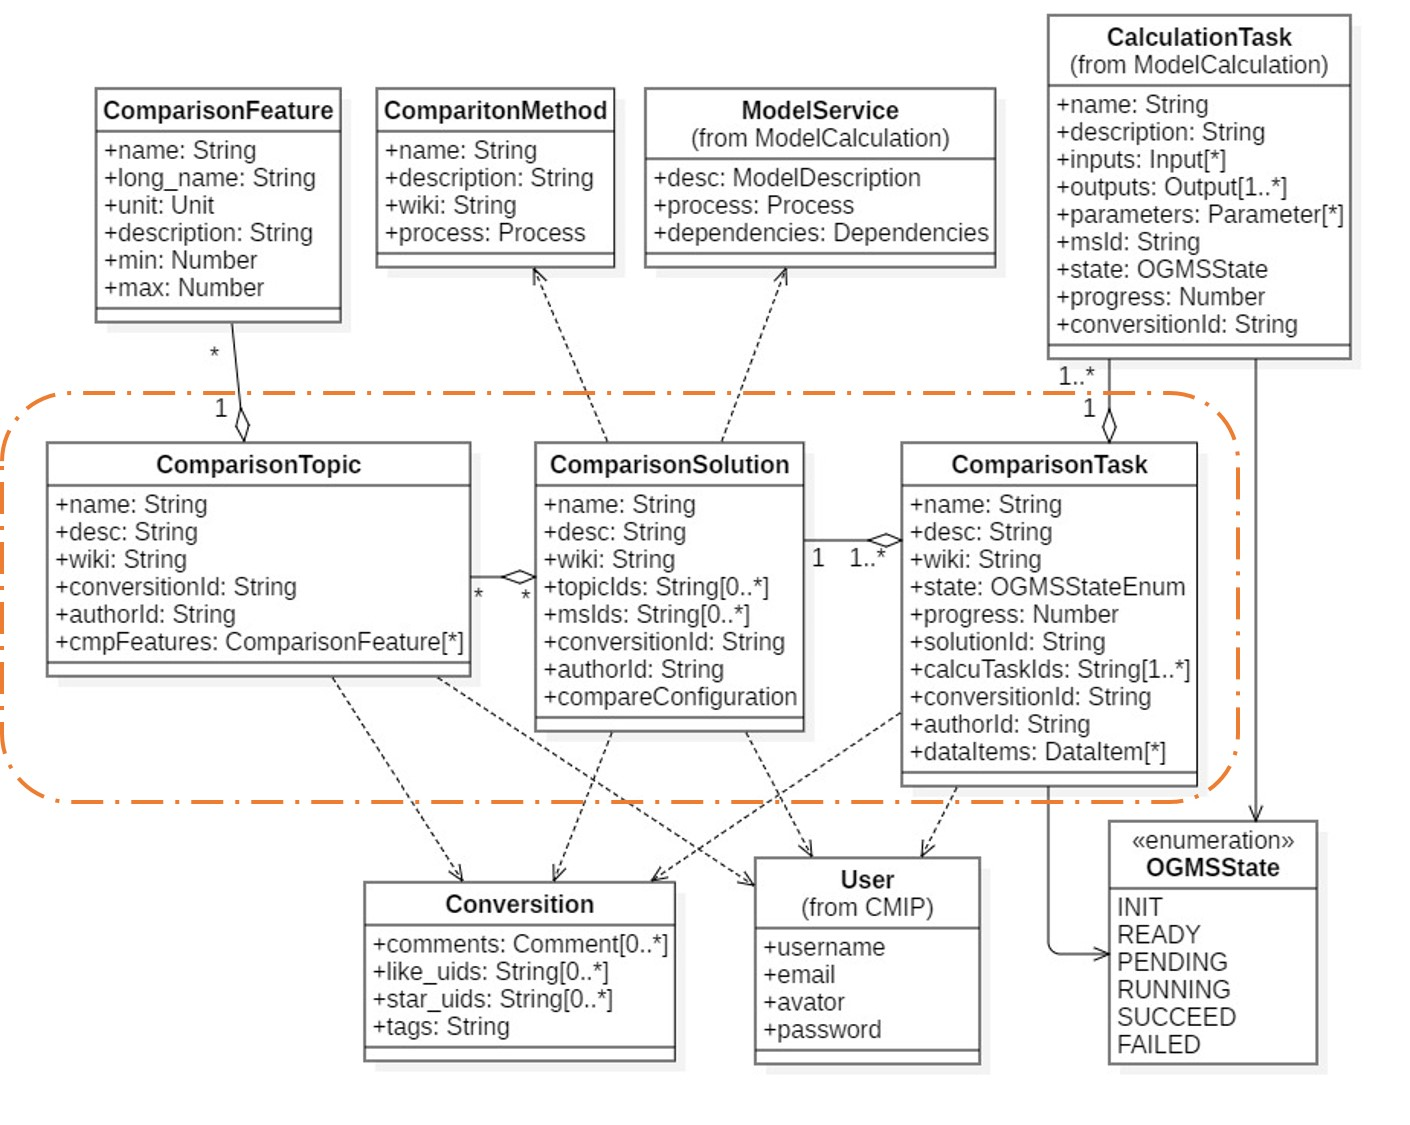
\includegraphics[width=1\textwidth]{jpg/ModelComparison!3-1-topic-solution-task_3}
    \caption{对比话题、对比方案和对比任务的接口设计UML图}
    \label{fig:ModelComparison!3-1-topic-solution-task_3}
\end{figure}

以植被生产力的对比为例,如表\ref{tab:topic-solution-task-example}所示,针对全球历史时期的植被生产力创建一个对比话题,对比要素包括有GPP、NPP、NEP等,这一个话题关联两个对比方案,他们的对比参与者相同,都是IBIS、Biome-BGC和LPJ三个模型,第一个方案在观测站点尺度开展对比,它使用的对比方法包括统计学和可视化两大类,通过配置不同的观测站点数据可以对应231个对比任务;第二个方案研究的是全球尺度,它使用的对比方法只有可视化对比方法,通过配置全球网格输入数据创建一个相应的对比任务。这样的三层抽象使对比方案可共享与重用,简化了模型对比的难度,并将最后的对比结果公开发布为服务,使对比过程公开透明,更加具有可信度。

% TODO 从 pdf 导入吧
\begin{table}
    \centering
    \caption{针对全球植被生产力评估的对比话题、对比方案和对比任务}
    \label{tab:topic-solution-task-example}
    \begin{threeparttable}
        \begin{tabular}{l | l | l | l | l }
            \Xhline{1.5pt}
            \multicolumn{2}{c}{\makecell[b]{对比话题}} & \multicolumn{2}{|c|}{\makecell[b]{对比方案}} & \multicolumn{1}{l}{\makecell[b]{对比任务}} \\
            \hline
            模拟情景 & 对比要素 & \makecell{对比参与者} & \makecell{对比方法} & 数据区域 \\
            \Xhline{1.5pt}
            \multirow{3}{*}{历史情景} & \multirow{3}{2cm}{GPP \quad NPP \quad NEP\ } & \multirow{3}{*}{\makecell{IBIS\\Biome-BGC\\LPJ}} & \multirow{2}{*}{\makecell{统计学对比方法\\可视化对比方法}} & \multirow{2}{*}{231个观测站点} \\
            &&&&\\
            \cline{4-5}
            &  &  & 可视化对比方法 & 全球网格点 \\
            \Xhline{1.5pt}
        \end{tabular}
    \end{threeparttable}
\end{table}

\section{对比科学工作流引擎}
\subsection{对比流程分析和归纳}
图~\ref{fig:workflow-example}展示了传统方法在本地进行对比时的流程,整个流程可以概括为“模型计算——数据重构——结果对比”三步。模型计算过程中对比参与者同时输入数据启动运行;数据重构过程将运算结果转换为标准化数据;结果对比过程使用脚本分析。当改变数据集或者加入新的对比参与者时整个对比流程都不会发生变化。

\begin{figure}[!htbp]
    \centering
    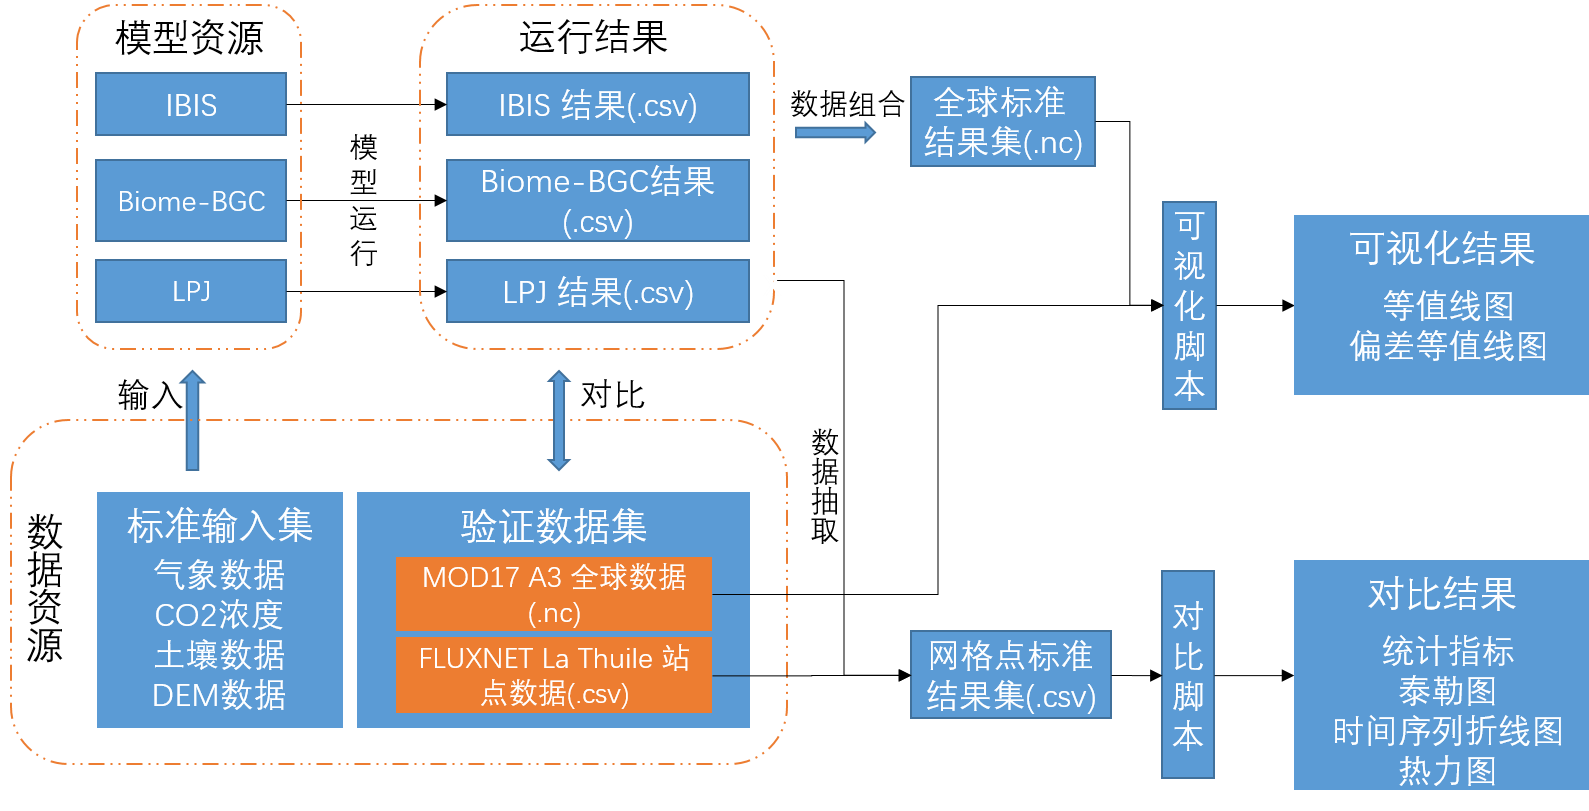
\includegraphics[width=1\textwidth]{workflow-example}
    \caption{以IBIS、Biome-BGC、LPJ三个模型为例的对比流程}
    \label{fig:workflow-example}
\end{figure}

\subsection{对比自动化执行引擎}
% 流程创建:是对工作流过程的抽象表示,定义工作流执行时使用的资源,其依赖关系着重表达了各任务之间从数据生产者到数据消费者的流程,这些资源是指可执行网络服务、数据,对应对比方案
% 通过流程映射形成可执行的工作流实例,对应对比任务
% 工作流定义:工作流语言通常用XML这种形式化描述语言,表达组成流程的任务和任务之间的依赖关系,SWF没有标准语言,流程定义只能由各自的流程引擎解析执行
% 工作流执行:运行时建立网络资源之间的交互关系,将抽象工作流转换成可执行的工作流,建立任务和所需可用资源的映射关系
% 工作流活动之间的依赖主要表达了多个任务之间的逻辑结构和执行方式,包括顺序、并行、循环、条件
在微服务架构下,由于数据和服务位置分散,面临着难以集成的问题,科学工作流是服务集成的一个解决方案。 % 具体化,数据传输的流程
工作流管理联盟(Workflow Management Coalition,WfMC)将工作流定义为一类能够完全或者部分自动执行的经营过程,根据一系列过程规则,文档、信息、或任务能够在不同的执行者之间传递、执行。科学工作流是工作流的一种,它主要面向科学实验过程,以数据驱动,用来描述和控制科学实验和过程的执行~\cite{ludascher2006scientific}~\cite{Zhao2009Special}。

科学工作流的生命周期可归纳为一下三点:
\begin{enumerate}[(1)]
    \item \textbf{流程创建:}定义工作流执行时所参与的活动,以及数据在活动之间的流向关系,在本文中活动是指各种模型服务、数据重构服务和对比服务。创建出的工作流表达了数据从生产者到消费者之间的流向关系,但还不包括数据实体;
    \item \textbf{流程映射:}绑定活动所需要的数据实体,从而将工作流映射为可执行的工作流实例;
    \item \textbf{流程执行:}解析工作流中活动的依赖关系,并在网络环境下进行运算。
\end{enumerate}

根据上小结的总结,在对比过程中工作流模式固定,都由“模型计算——数据重构——结果对比”三步组成,所以本文不再通过图形化界面创建工作流,只需要通过选择对比参与者和对比方法就能够映射到这三部流程,可以通过第~\ref{sec:cmp-CSDL}设计的对比方案描述文档表达,流程创建对应对比方案(ComparisonSolution)的创建,流程映射对应对比任务(ComparisonTask)的创建,流程执行对应对比任务的执行。

\begin{figure}[!htbp]
    \centering
    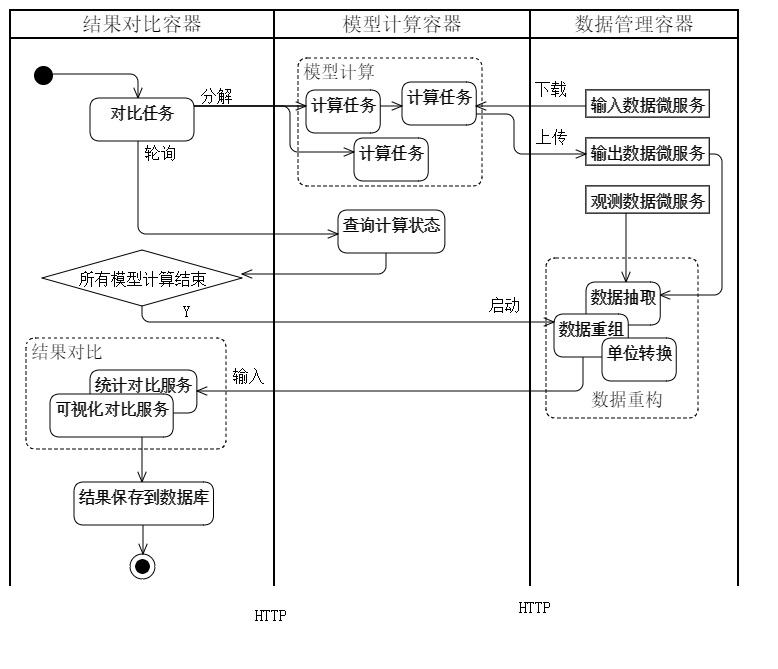
\includegraphics[width=1\textwidth]{jpg/ModelComparison!Activity1!3-4workflow_6}
    \caption{开放式对比科学工作流流程图}
    \label{fig:workflow}
\end{figure}

图~\ref{fig:workflow}展示了对比工作流的执行流程,整个对比流程包括:
\begin{enumerate}[(1)]
    \item 用户通过客户端提交并启动对比任务;
    \item 工作流引擎将对比任务分解为模型计算任务,分发给模型微服务;
    \item 模型微服务作为数据微服务的消费者,从数据管理容器上下载输入数据文件,当所有数据准备完成后启动模型开始计算;
    \item 工作流引擎通过轮询监控模型的运行进度;
    \item 当所有模型运行结束后,工作流引擎向数据管理容器发送启动请求,调用数据重构服务;
    \item 数据重构运行结束后开始调用对比脚本;
    \item 将对比结果保存到数据库中。
\end{enumerate}

通过对比工作流的驱动,保证了模型对比流程能够按部就班的开展,大大简化了用户操作的复杂性。

% 每一步都是在网络环境下,有频繁的数据传输交互
\section{本章小结}
开放式对比系统的构建有两个关键问题:一是如何设计一个开放式的对比框架,二是这些对比资源如何接入框架。对于问题一,本章从网络架构、服务容器和地理资源组件、对比业务、执行引擎四个角度进行了详细论述,设计的系统框架具有以下特点的:
\begin{enumerate}[(a)]
    \item 模型计算和对比可共享与重用;
    \item 模型计算和对比过程公开化;
    \item 模型和数据资源可扩展性地动态接入;
    \item 大规模计算场景下稳定可用;
    \item 以自动化实现其易用性。
\end{enumerate} 

对于问题二将在下一章详细论述。